\documentclass{article}
\usepackage{float}
\usepackage{graphicx}
\usepackage{fancyhdr}

\usepackage{geometry}
\geometry{margin=1in}
\setlength{\headheight}{49.4pt}
\pagestyle{fancy}
\fancyhf{}
\rhead{
    \centering
  \begin{tabular*}{\textwidth}{@{\extracolsep{\fill}}ccc}
    \small University of Florida & \textbf{\small EEL3111C - Circuits} & \small Rottenberg, Cole Harrison\\
    \small Electrical \& Computer Engineering Dept. & \small Lab 8: Diode Applications & \small Class \#: 20931 \\
    \small Page \thepage & \small Revision: 0 & \small \today \\
  \end{tabular*}
}

\begin{document}
% I need a bold horizontal line

\begin{center}
    \hrule
    \vspace{0.2cm}
    \textbf{\large REQUIREMENTS NOT MET}
    \vspace{0.2cm}
    \hrule
\end{center}
% Bullet points on what was not met
\begin{itemize}
    \item All Requirements were met.
\end{itemize}

\begin{center}
    \hrule
    \vspace{0.2cm}
    \textbf{\large PROBLEMS ENCOUNTERED}
    \vspace{0.2cm}
    \hrule
\end{center}
% More Bullet points with filler text
\begin{itemize}
    \item No problems were encountered.
\end{itemize}

\begin{center}
    \hrule
    \vspace{0.2cm}
    \textbf{\large INTRODUCTION}
    \vspace{0.2cm}
    \hrule
\end{center}

We explore the characteristics of diodes, how voltage differences affect current flow and how to use diodes to create a half wave rectifier. We also explore the use of comparators and how to use them to create a circuit that can detect when a voltage is above or below a certain threshold.

\begin{center}
    \hrule
    \vspace{0.2cm}
    \textbf{\large DISCUSSION}
    % A horizontal line here
    \vspace{0.2cm}
    \hrule
\end{center}

\textbf{\large8.5 Pre-Lab Requirements:}

\textbf{8.5.1 LTspice Simulations:}
\begin{enumerate}
    \item Set the input to a 1 kHz, 5 V amplitude
sine wave and run a transient simulation with a stop time of 1m (.tran 1m)
and plot the input and output. To use the 1N4148 diode model, right click on
the diode after placing it, Pick New Diode, and then choose the 1N4148 model
(Mfg. OnSemi). Save an image of the circuit and the plot of the input and
output voltage for submission to canvas.
    \begin{figure}[H]
        \centering
        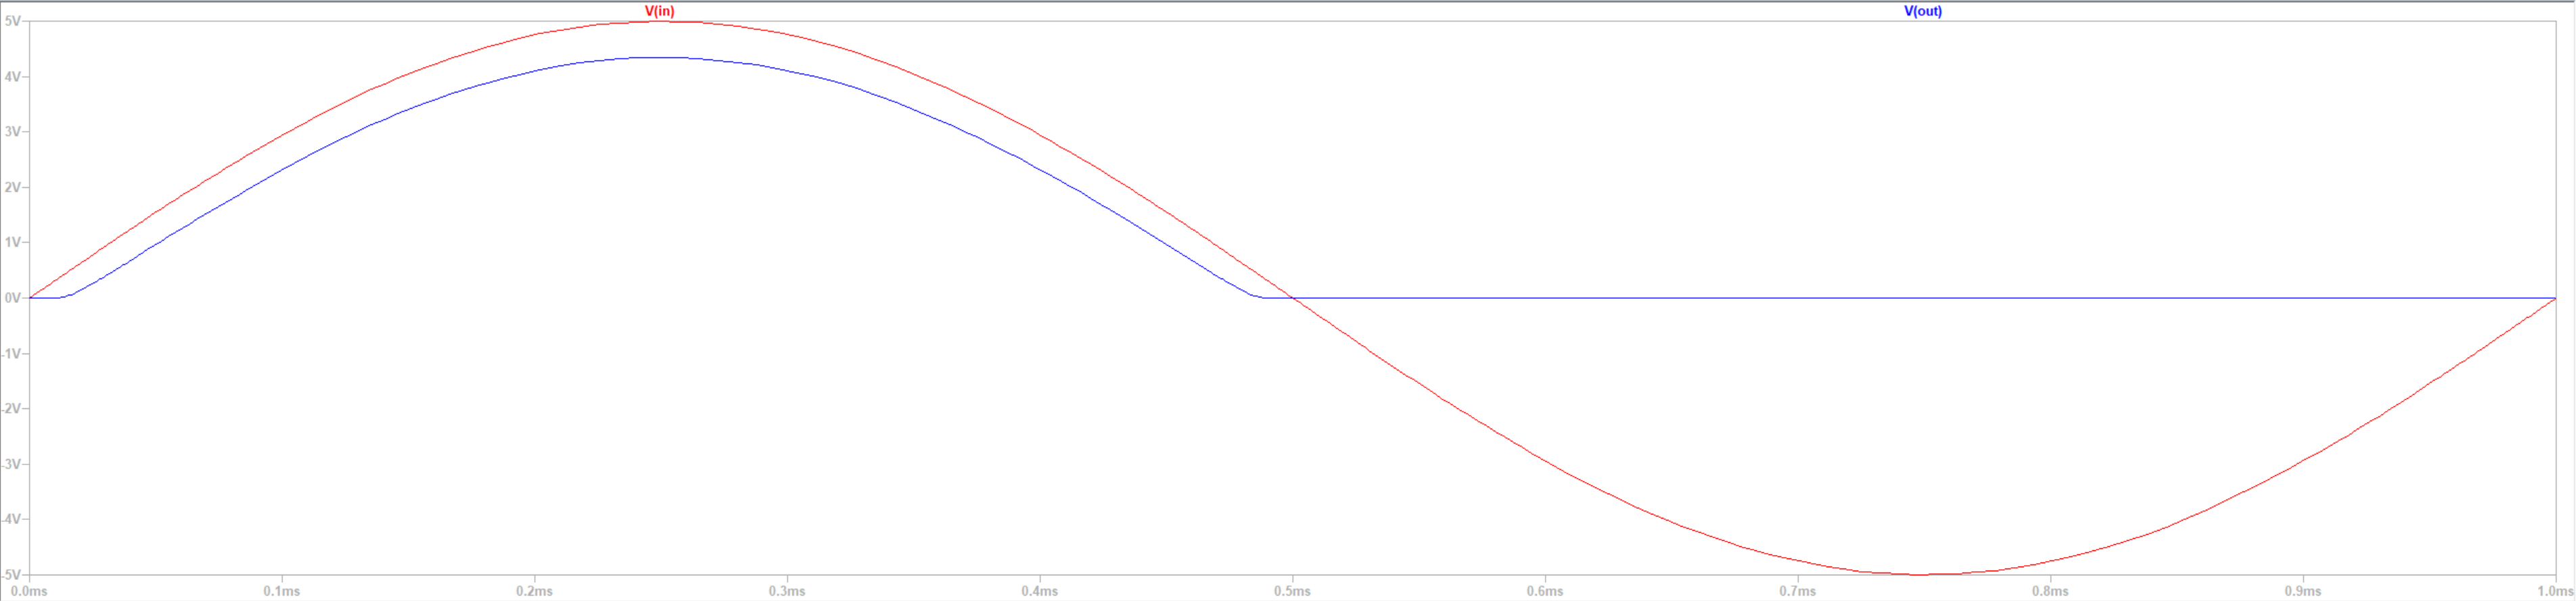
\includegraphics[width=0.75\textwidth]{fig8_2_a.png}
        \caption{HALF WAVE RECTIFIER PLOT} 
        \label{fig:half_wave_rectifier}
    \end{figure}
    \begin{figure}[H]
        \centering
        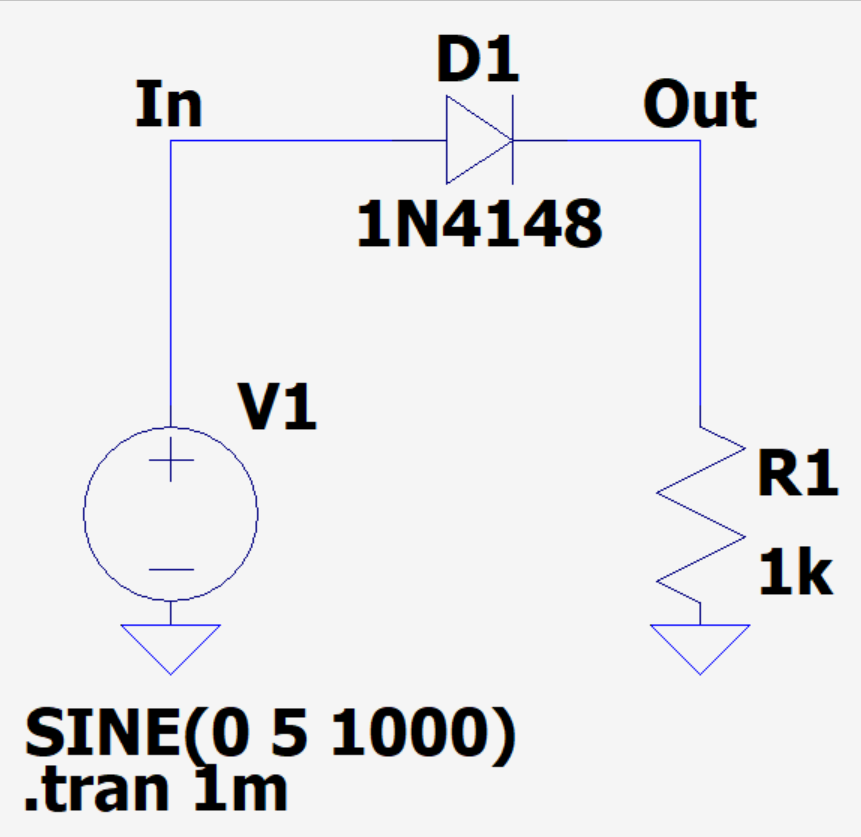
\includegraphics[width=0.75\textwidth]{circuit8_2_a.png}
        \caption{HALF WAVE RECTIFIER CIRCUIT} 
        \label{fig:half_wave_rectifier_circuit}
    \end{figure}
    \item Build the circuit in Figure 8.3 (a). Set the input to a 100 kHz, 5 V amplitude
sine wave and run a transient simulation with a stop time of 50u (.tran 50u)
and step through possible capacitor values using the following spice directive:
    \begin{figure}[H]
        \centering
        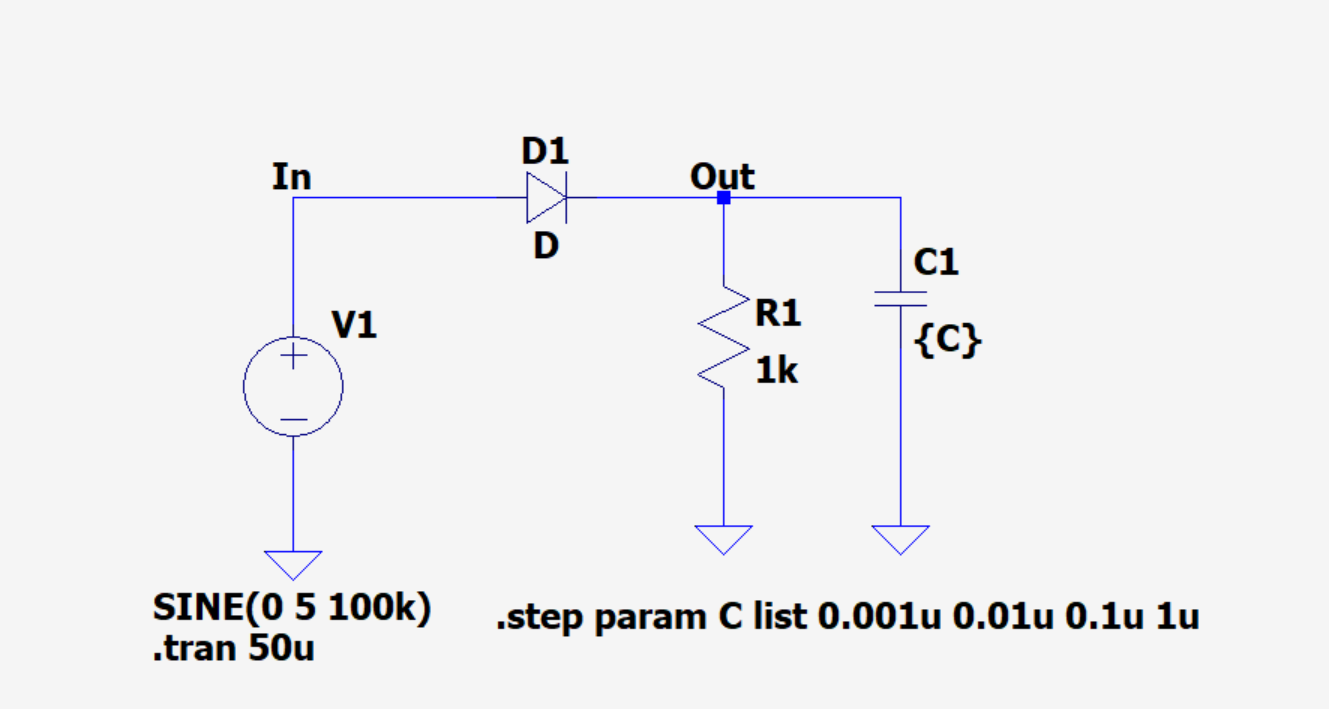
\includegraphics[width=0.75\textwidth]{circuit8_3a.png}
        \caption{HALF WAVE RECTIFIER CIRCUIT WITH  CAPACITOR} 
        \label{fig:HALF WAVE RECTIFIER CIRCUIT WITH CAPACITOR}
    \end{figure}

    \begin{figure}[H]
        \centering
        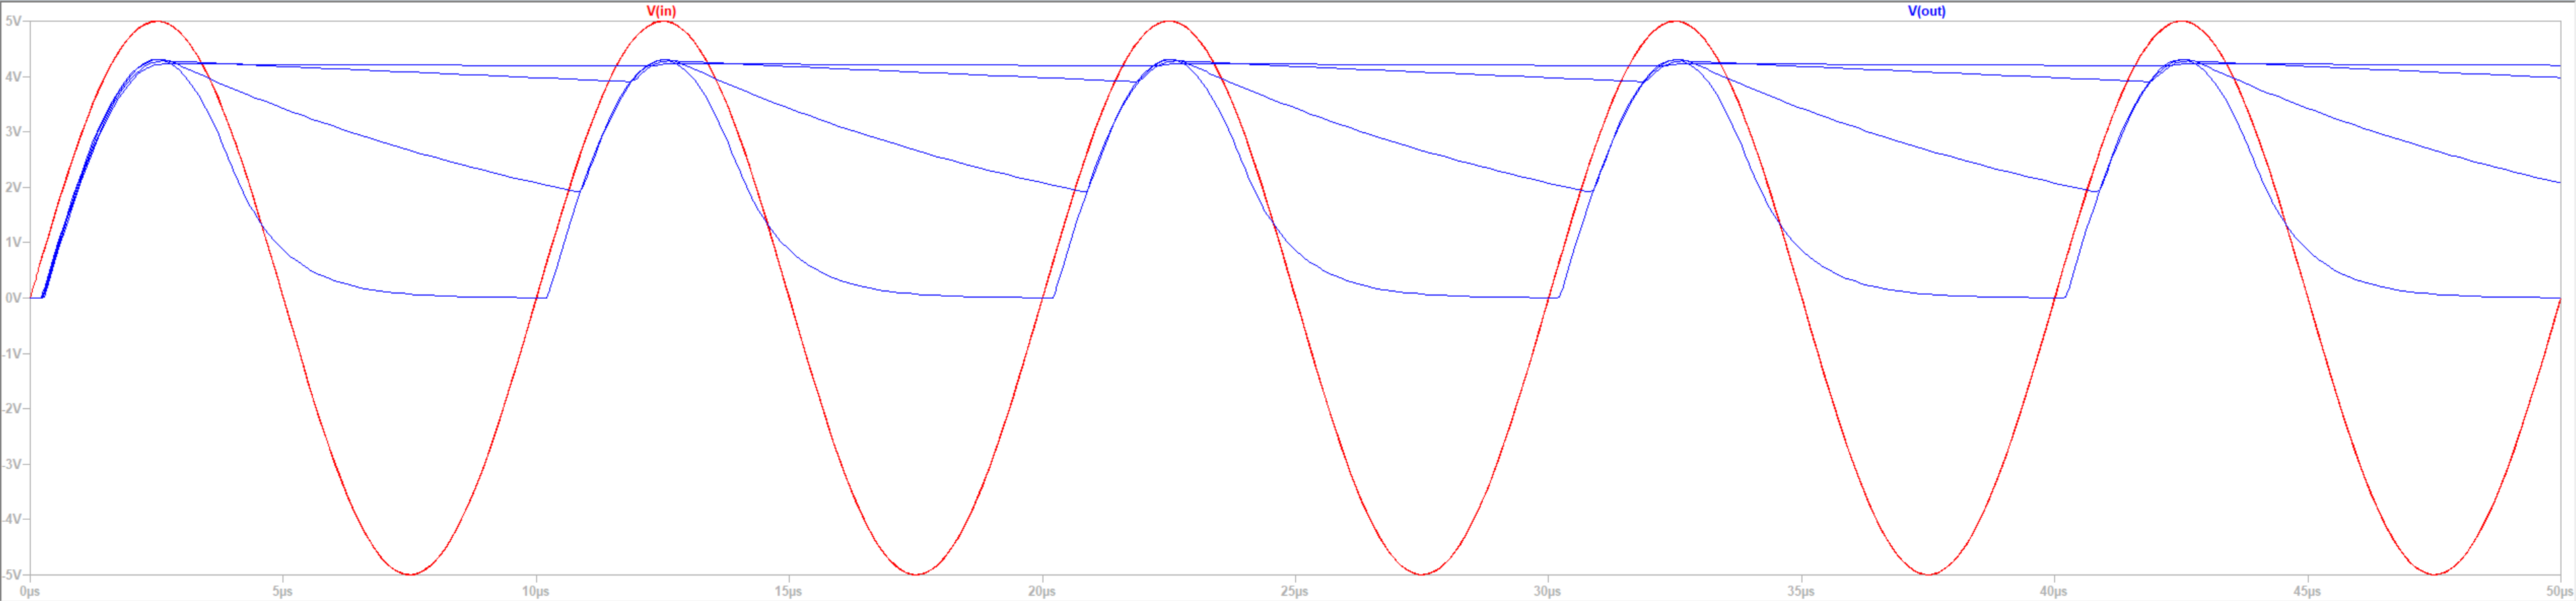
\includegraphics[width=0.75\textwidth]{plot8_3a.png}
        \caption{HALF WAVE RECTIFIER CIRCUIT WITH CAPACITOR PLOT}
        \label{fig:half_wave_rectifier_plot}
    \end{figure}
    \item Build the circuit in Figure 8.4. Use the default LED model in LTSpice, and
download "slcj016.zip" file from Canvas "Lab Related Files" folder for the LM393
comparator model. Don’t use the "slcj016b.zip" for the comparator model from 
TI because it’s a newer model that doesn’t work for input higher than (Vcc-2V).
Power the LM393 with +/-5 V. Set the input voltage to a 1 kHz, 5 V amplitude
sine wave and run a transient solution with a stop time of 2m (.tran 2m). Plot
the input voltage and the current through each diode. Save an image of the
circuit and the plot for submission to canvas
    \begin{figure}[H]
        \centering
        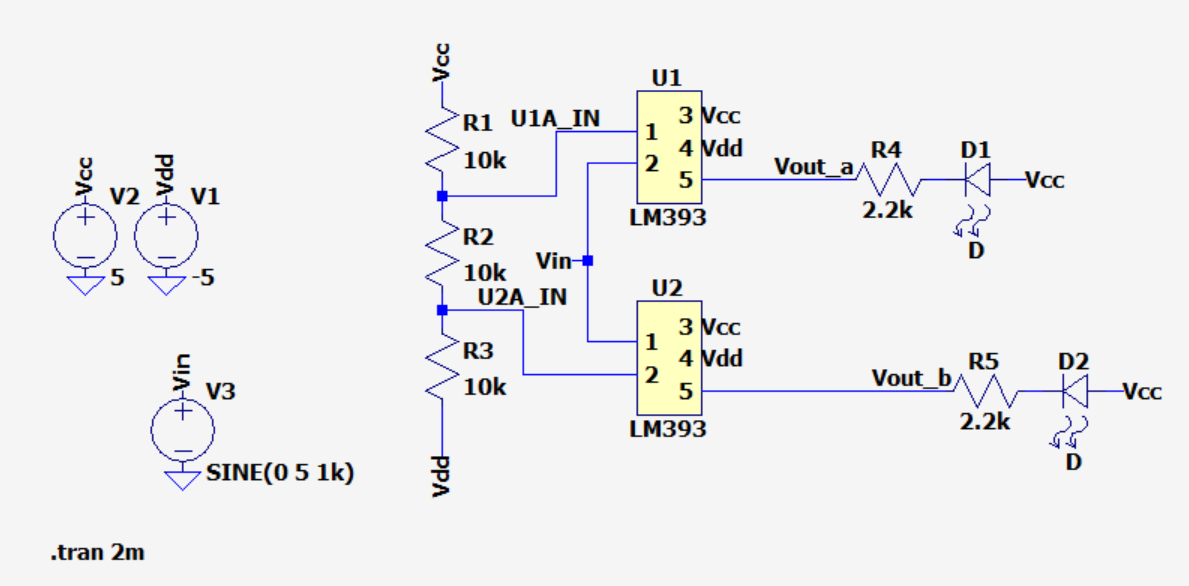
\includegraphics[width=0.75\textwidth]{circuit8_4.png}
        \caption{COMPARATOR CIRCUIT} 
        \label{fig:comp-circuit}
    \end{figure}

    \begin{figure}[H]
        \centering
        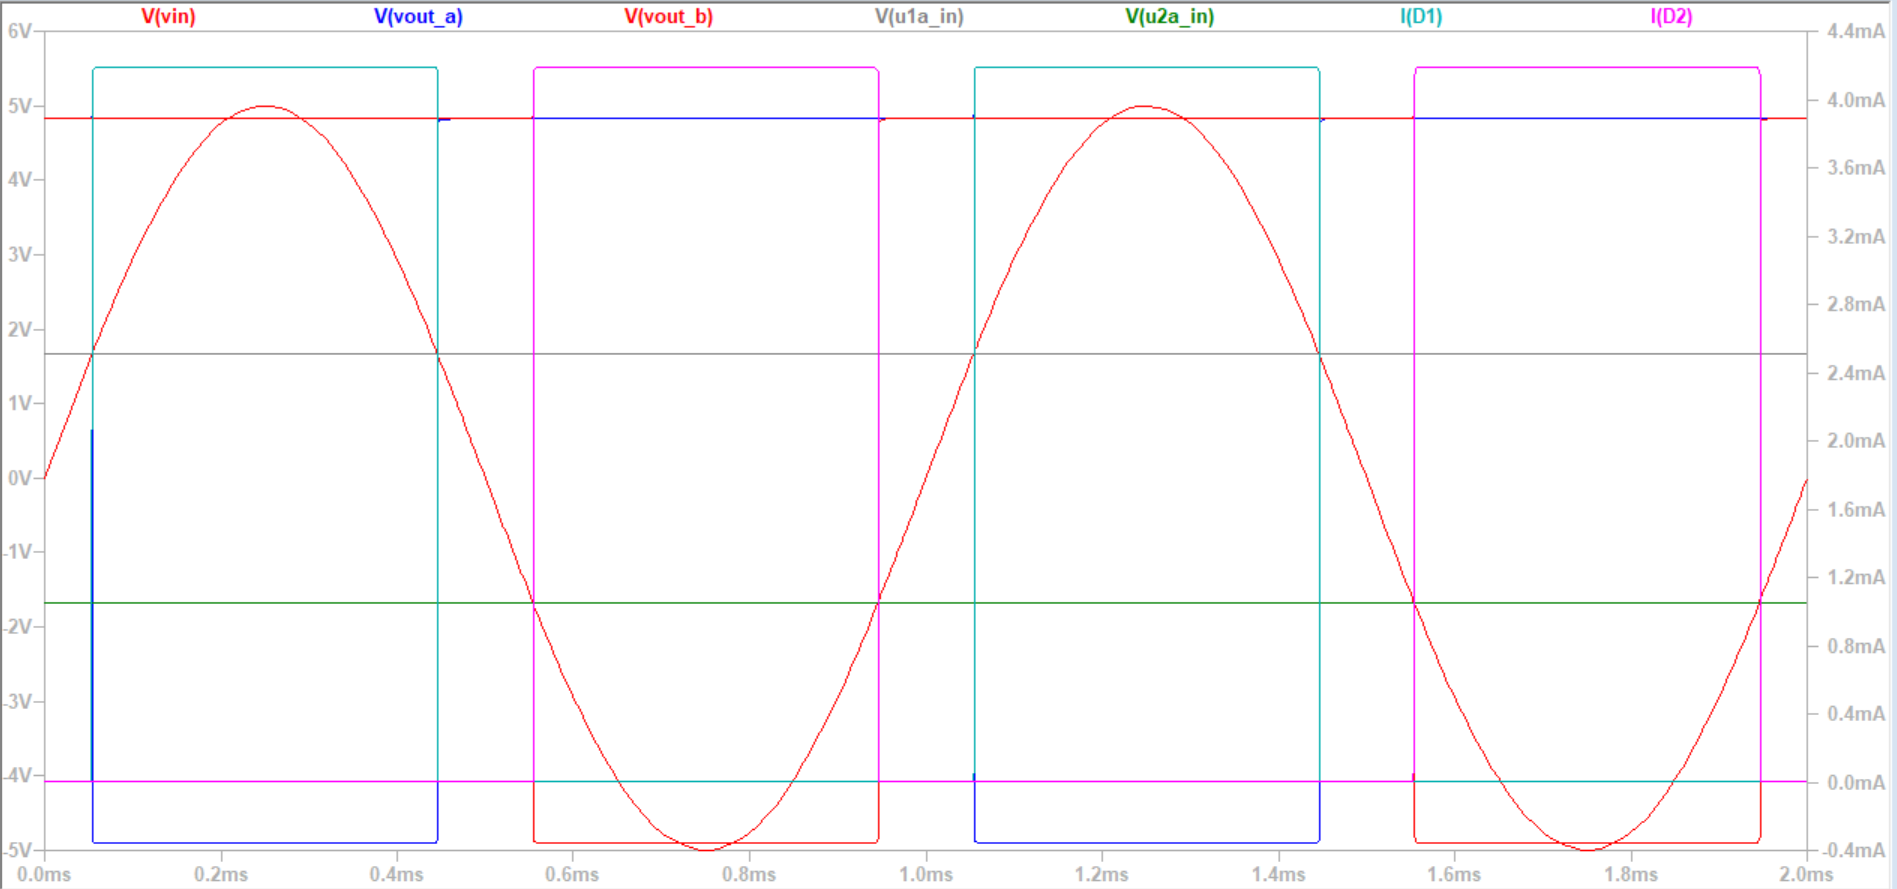
\includegraphics[width=0.75\textwidth]{plot8_4.png}
        \caption{COMPARATOR PLOT} 
        \label{fig:comp-plot}
    \end{figure}
    \item Build the circuit in Figure 8.7. Power the LM393 and TLV272 with +/-5 V.
Set the input voltage to a 1kHz, 0.1 V amplitude sine wave and run a transient
solution with a stop time of 2m. Choose the value for R1, 10k pot, so that
the diodes conduct current and illuminate. Plot the input voltage, output of
the op amp, positive and negative inputs to the comparator, and the current
through both LEDs. (6 items total). Save an image of the circuit and the plot
for submission to canvas.
    \begin{figure}[H]
        \centering
        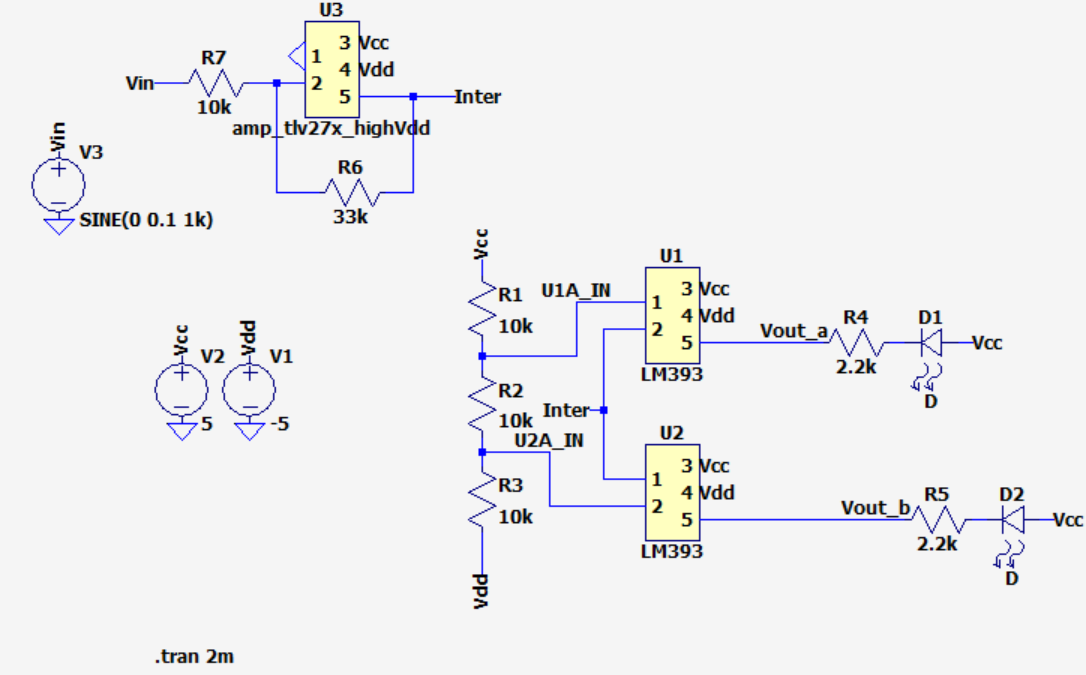
\includegraphics[width=0.75\textwidth]{circuit8_7.png}
        \caption{COMPARATOR CIRCUIT WITH OP-AMP} 
        \label{fig:comp-circuit-op-amp}
    \end{figure}

    \begin{figure}[H]
        \centering
        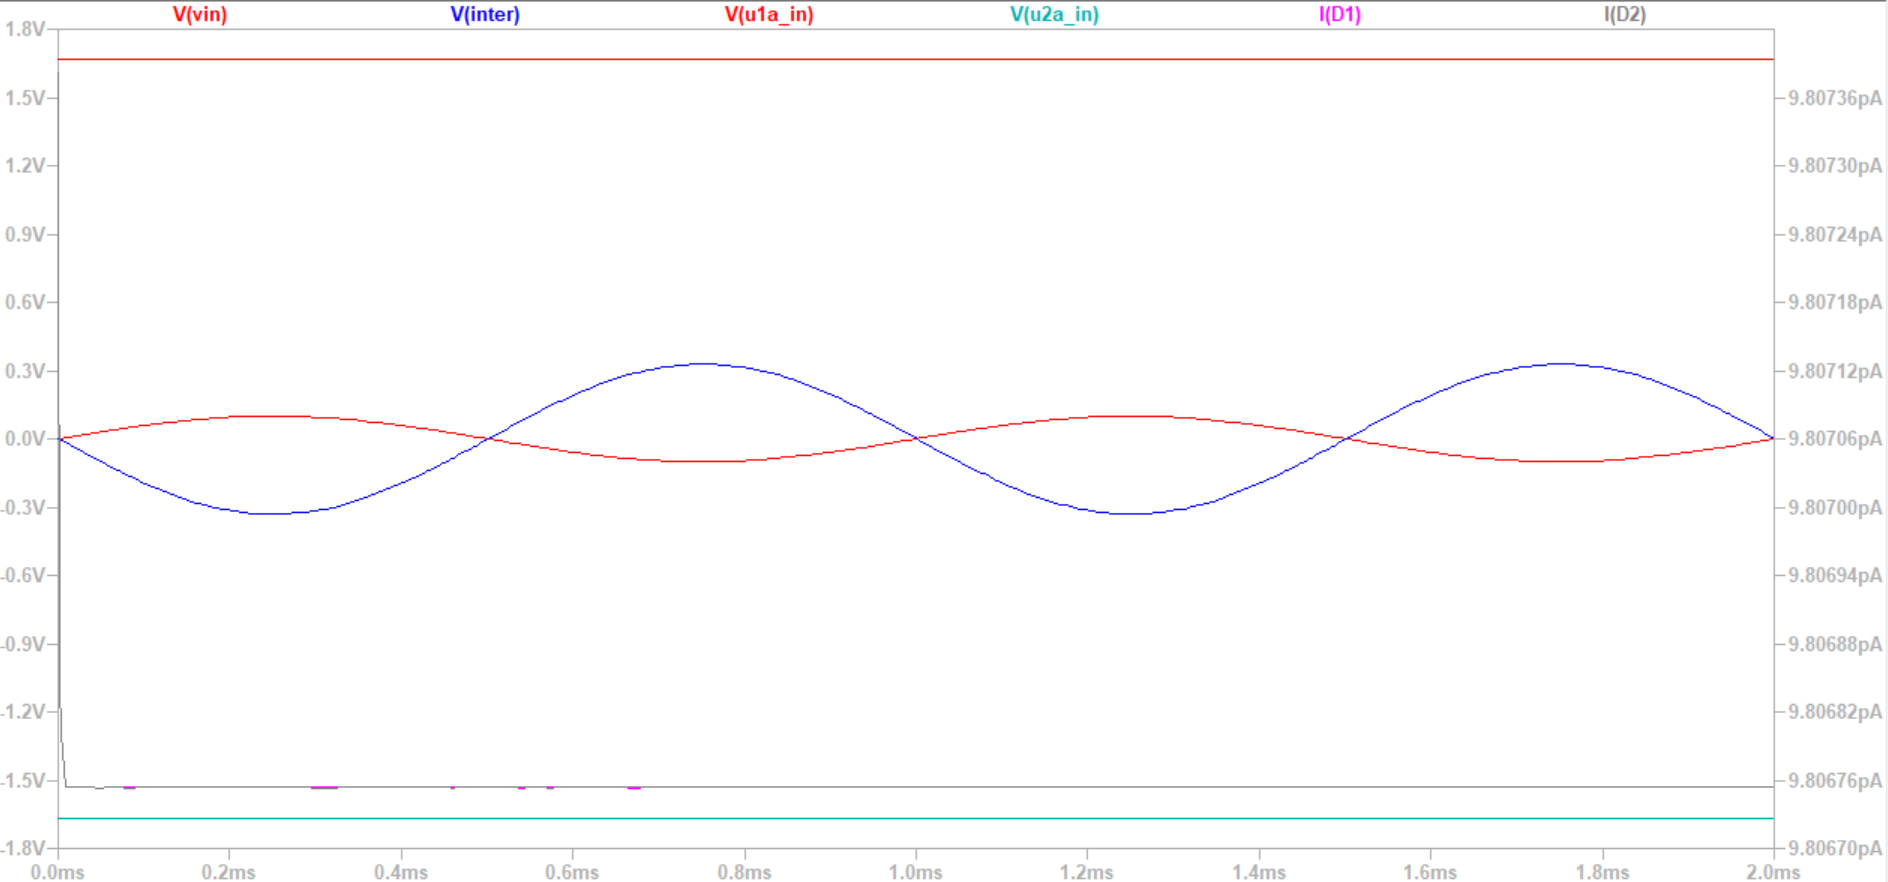
\includegraphics[width=0.75\textwidth]{plot8_7.png}
        \caption{COMPARATOR PLOT WITH OP-AMP} 
        \label{fig:comp-plot-op-amp}
    \end{figure}
\end{enumerate}
\textbf{8.5.2 Breadboard Implementation:}
\begin{enumerate}
    \item Build the circuit in Figure 8.4 on the breadboard. The following plot shows the o-scope output.
    \begin{figure}[H]
        \centering
        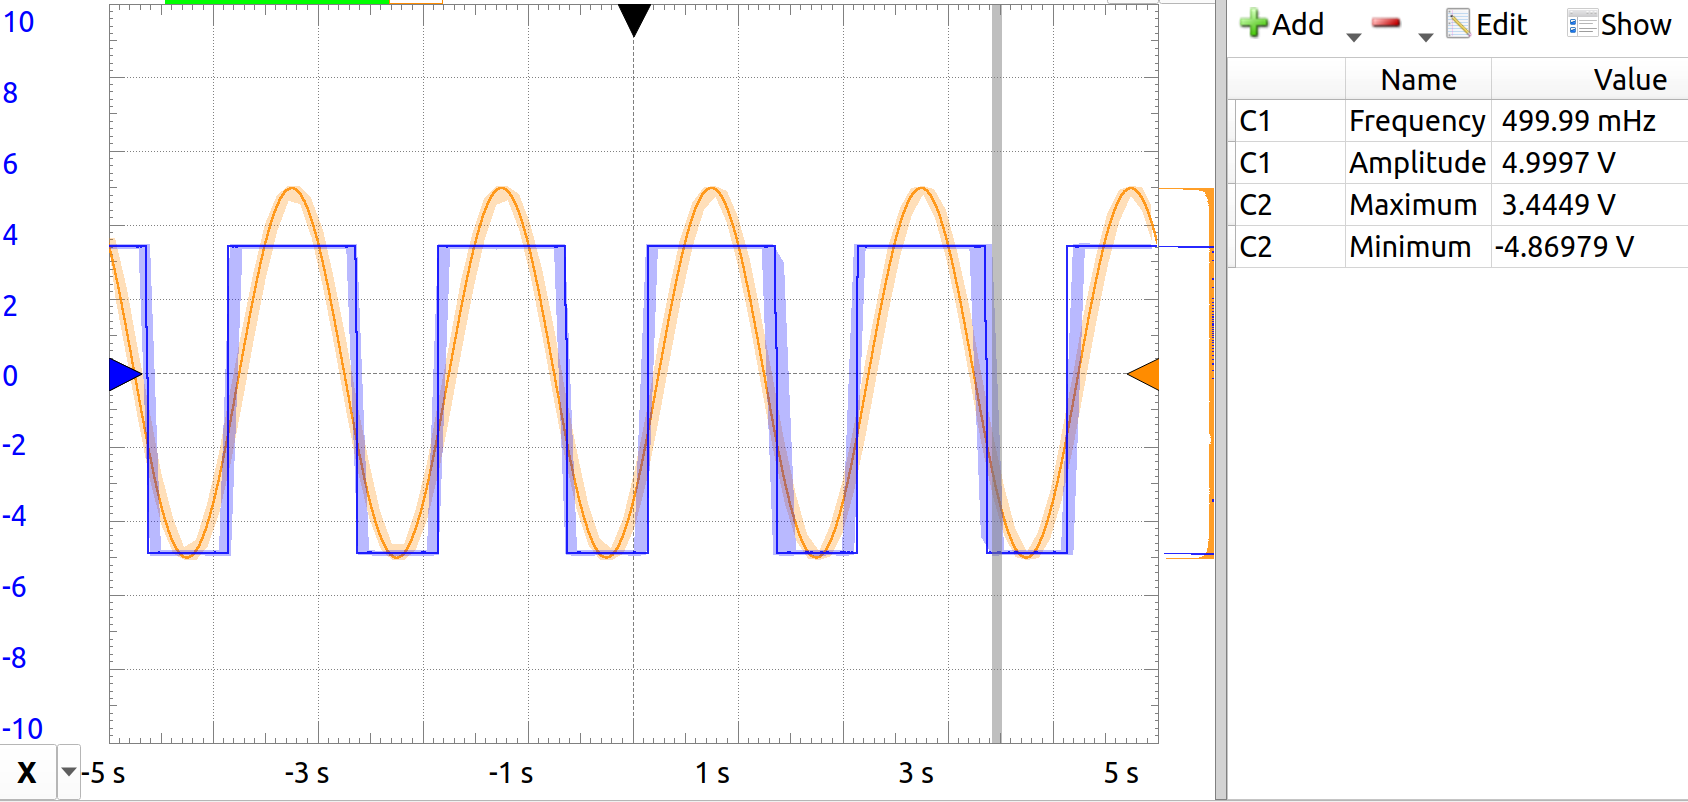
\includegraphics[width=0.75\textwidth]{inlab_1.png}
        \caption{COMPARATOR PLOT PHYSICAL} 
        \label{fig:comp-plot-phys}
    \end{figure}
    \item Build the circuit from Section 8.5.1 - Item 1. Plot the input and output on the o-scope and save an image of the display. 
    \begin{figure}[H]
        \centering
        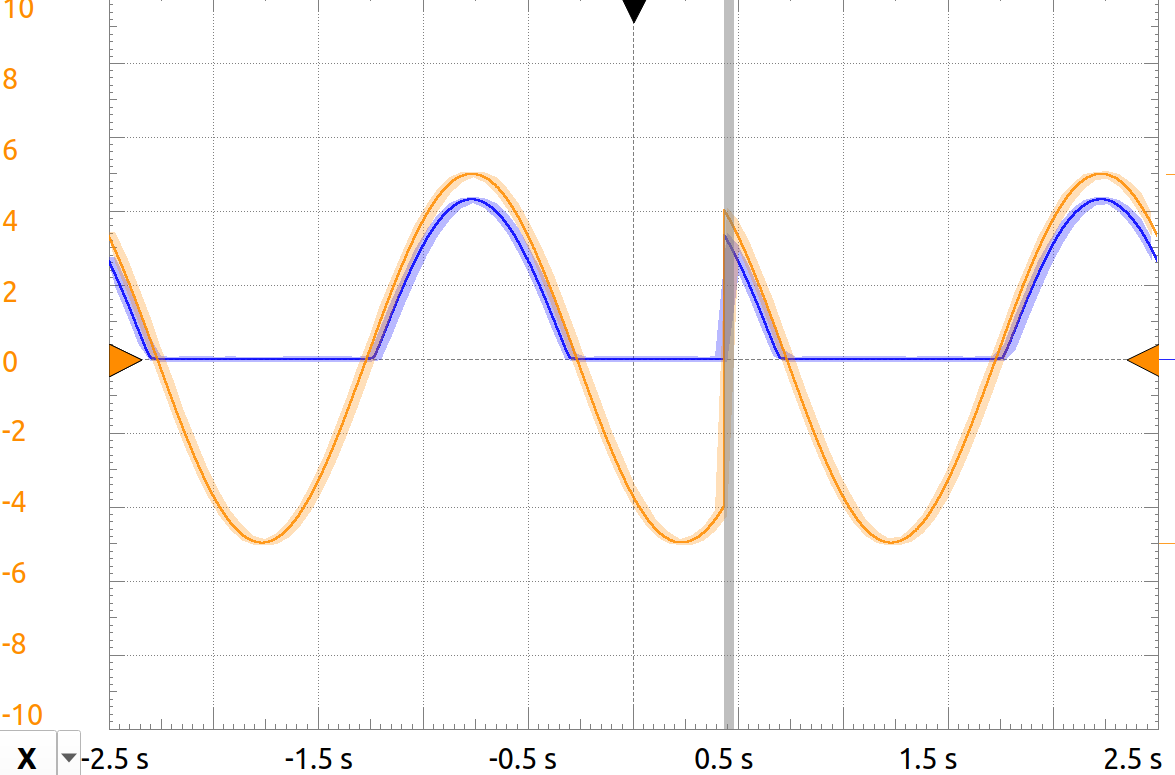
\includegraphics[width=0.75\textwidth]{inlab_2.png}
        \caption{8.5.1 PLOT PHYSICAL} 
        \label{fig:851-plot-phys}
    \end{figure}
    \item Build two version of the circuit from Subsection 8.5.1 - Item 2, one with where
the capacitance is 0.1 uF and the other is 0.01 uF. Plot the outputs of both
circuits on the o-scope and save an image of the display.
    \begin{figure}[H]
        \centering
        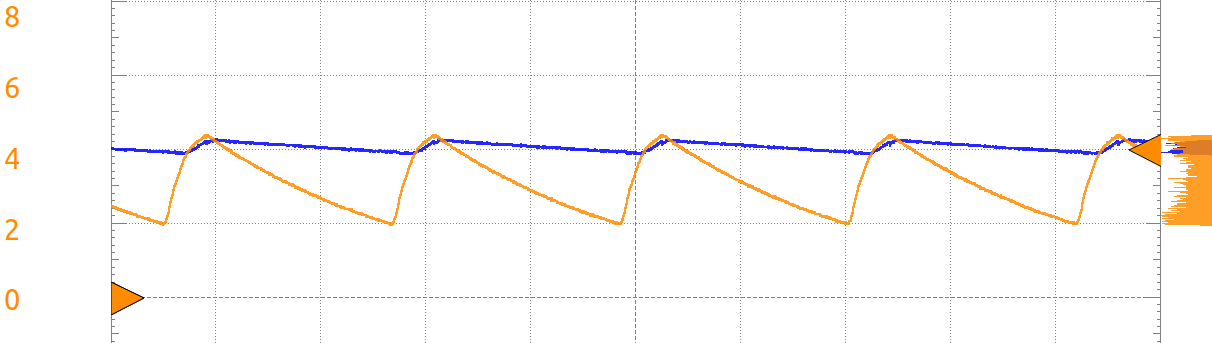
\includegraphics[width=0.75\textwidth]{inlab_3.png}
        \caption{DIFFERENCE IN CAPS PLOT PHYSICAL} 
        \label{fig:diff-plot-phys}
    \end{figure}
    \item Build the circuit from Subsection 8.5.1 - Item 4. Set the input to a 0.5 Hz, 0.1
V amplitude sine wave. Vary the potentiometer, increase the gain, so that the
LEDs illuminate when the op amp output is greater than the reference voltages.
Plot the output of the gain amplifier and the output of either comparator on
the o-scope and save an image of the display
    \begin{figure}[H]
        \centering
        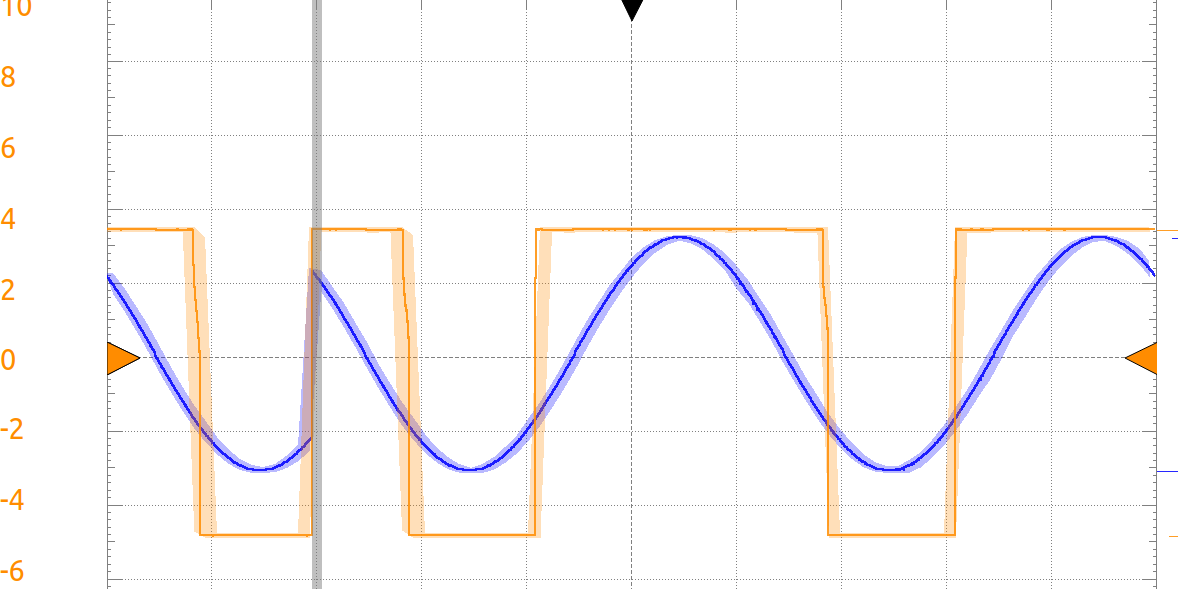
\includegraphics[width=0.75\textwidth]{inlab_4.png}
        \caption{POTENTIOMETER PLOT PHYSICAL} 
        \label{fig:pot-plot-phys}
    \end{figure}


\end{enumerate}
\pagebreak
\begin{center}
    \hrule
    \vspace{0.2cm}
    \textbf{\large CONCLUSION}
    % A horizontal line here
    \vspace{0.2cm}
    \hrule
\end{center}

Comparitively, we first explore the first circuit brought to attention in the lab, the half-wave rectifier. A rectifier circuit is used to convert AC to DC typically with the use of diodes.
The circuit can be viewed on Figure~\ref{fig:half_wave_rectifier_circuit}, The diode will only allow current to flow forwards as seen in \textbf{Figure \ref{fig:half_wave_rectifier_plot}}. The second circuit introduces a capacitor to the circuit. The capacitor will charge up to the peak voltage of the input signal and then discharge through the load resistor. This charging effect essentially smooths the output. In the half-wave rectifier with the capacitor, we can see the voltage level not dropping fully to zero, or dropping at a slower rate in \textbf{Figure \ref{fig:half_wave_rectifier_plot}}.
The third circuit mentioned was the comparator circuit. The comparator circuit is used to compare two voltages and output a digital signal based on the comparison. The circuit can be viewed on \textbf{Figure~\ref{fig:comp-circuit}}. The output of the comparator is either high or low depending on the voltage of the input signal. This would the drive the LEDs.
The fourth circuit is a comparator circuit with an op-amp. The op-amp is used to amplify the input signal. The circuit can be viewed on \textbf{Figure~\ref{fig:comp-circuit-op-amp}}. The output of the op-amp is then fed into the comparator circuit. The output of the comparator circuit is then used to drive the LEDs. The LEDs will light up when the voltage of the input signal is greater than the reference voltage. The reference voltage is set by the potentiometer. The potentiometer is used to adjust the reference voltage. The circuit can be viewed on \textbf{Figure~\ref{fig:pot-plot-phys}}.
\end{document}